\begin{problem}{4} ~\\
(a) To answer every query with no addition, we need to store all possible sub arrays of A. The number of sub arrays of a n*n array is $\binom n2 * \binom n2 = \theta(n^4)$. This proves both the upper and lower bounds.\\
\\
(b) With the budget of one addition, using divide and conquer can reduce the number of sums needed to store.\\
\\
First, we divide the array into two equal halves on one dimension and store each suffix-sum of A' and each prefix-sum of A''. If a query requests the sum of a sub array which crosses the line of division, then we are done (Figure 1). If the required sub array lies on one side (A' or A'') of the division line, we divide the sub array of the side into two equal halves on the other dimension (Figure 2). This process is recursively repeated and there's an equation can express it:\\
$$T(N) = 2T(\frac{N}{2}) + \theta(N^\frac{3}{2})$$ \\
In the equation, $N = n^2$ is the size of the problem. $N^\frac{3}{2}$ is the number of sums needed to store for the current problem size. Using Master Theorem, we know that T(N) = $\theta(N^\frac{3}{2})$. Therefore, $S_1(n) = O(n^3)$

\begin{figure}[H] 
\centering 
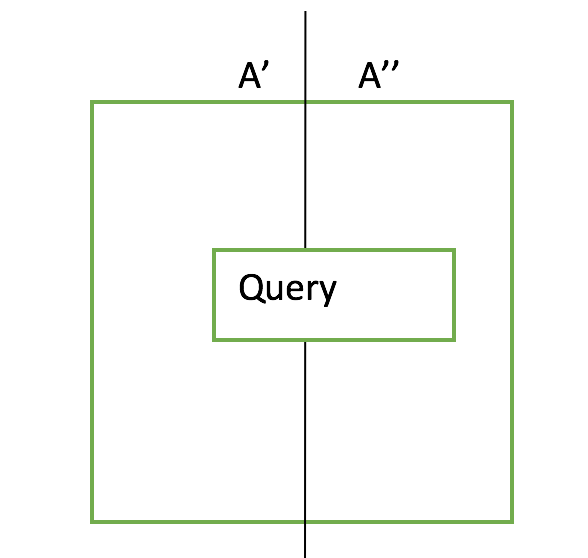
\includegraphics[width=0.5\columnwidth]{1}
\caption{query across the line}
\end{figure}

\begin{figure}[H] 
\centering 
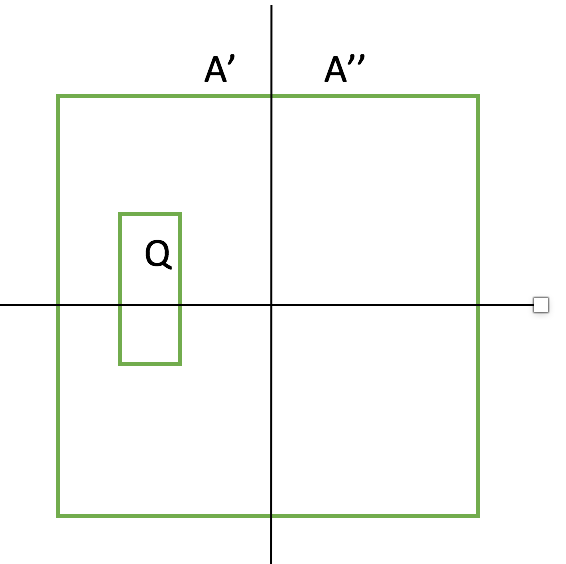
\includegraphics[width=0.5\columnwidth]{2}
\caption{query lies on one side}
\end{figure}
(c) We can achieve $O(n^2\log{n})$ using 2n-1 additions. From class, we know that each one-addition 1D problem can be solved in $O(n\log{n})$. We leverage this solution on the 2D problem.\\
\\
We reduce the 2D n*n problem into n 1D problems, each of the 1D problems needs $O(nlogn)$ space. There are n 1D problems, so the total space is $O(n^2logn)$. Each 1D problem needs one addition. To add up n 1D problems, we need n-1 additions. Therefore, the total number of additions is 2n-1.
\end{problem}